\section{Arquitectura Kappa}

\subsection{Descripción General}
La Arquitectura Kappa es un patrón de arquitectura de procesamiento de datos propuesto por Jay Kreps en 2014 como una 
simplificación de la Arquitectura Lambda. Su objetivo principal es unificar el procesamiento por lotes y en 
tiempo real en un único flujo de datos, eliminando la necesidad de mantener códigos separados para estos dos tipos de procesamiento. 
La Arquitectura Kappa se basa en la premisa de que todo es un flujo de datos (Stream) y que el reprocesamiento 
se puede lograr simplemente reproduciendo este flujo desde el principio.

\subsection{Componentes Principales}

\subsubsection{Stream Store Layer}
\begin{itemize}
    \item Actúa como un registro inmutable de todos los eventos de datos entrantes.
    \item Permite la reproducción de datos históricos para reprocesamiento cuando se actualiza la lógica de procesamiento.
\end{itemize}

\subsubsection{Stream Processing Layer}
\begin{itemize}
    \item Ingiere datos en tiempo real desde diversas fuentes.
    \item Procesa estos datos utilizando un sistema de procesamiento de streams.
    \item Aplica la lógica de negocio y las transformaciones necesarias a los datos entrantes.
\end{itemize}

\subsubsection{Serving Layer}
\begin{itemize}
    \item Almacena los resultados procesados del stream.
    \item Proporciona acceso de baja latencia a los resultados.
\end{itemize}

\newpage
\subsubsection{Vista Logica}
\begin{figure}[h]
\centering
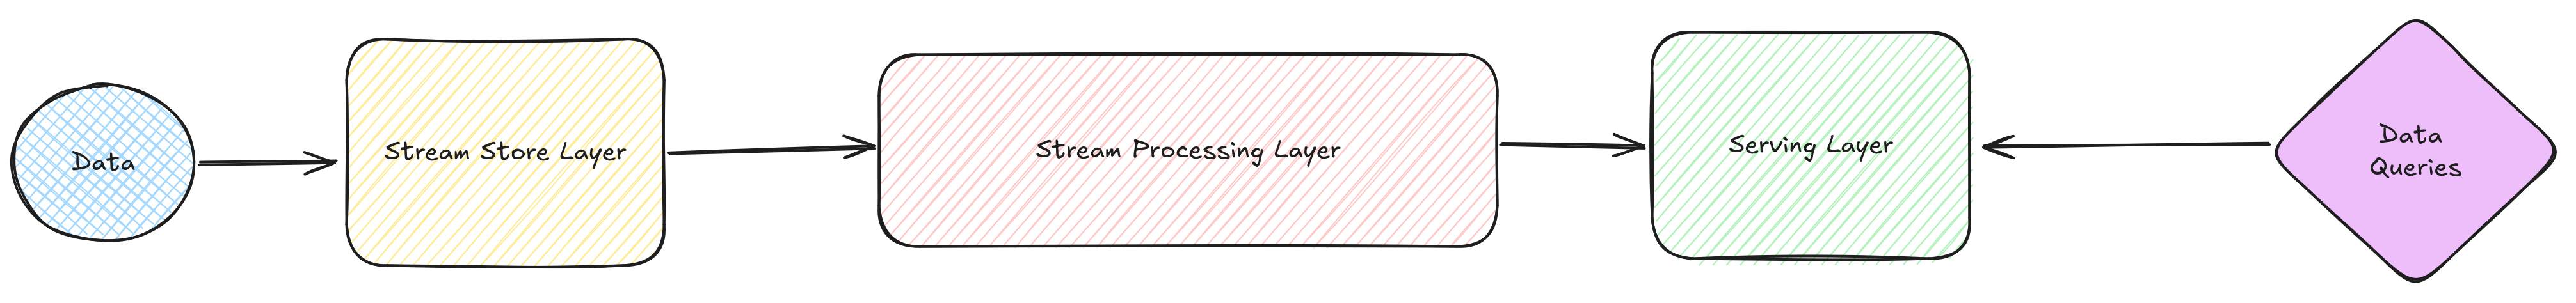
\includegraphics[width=0.8\textwidth]{teorico/kappa.png}
\caption{Diagrama de la Arquitectura Kappa}
\label{fig:arquitectura_kappa}
\end{figure}

\subsubsection{Implementacion Tipica}
\begin{figure}[h]
\centering
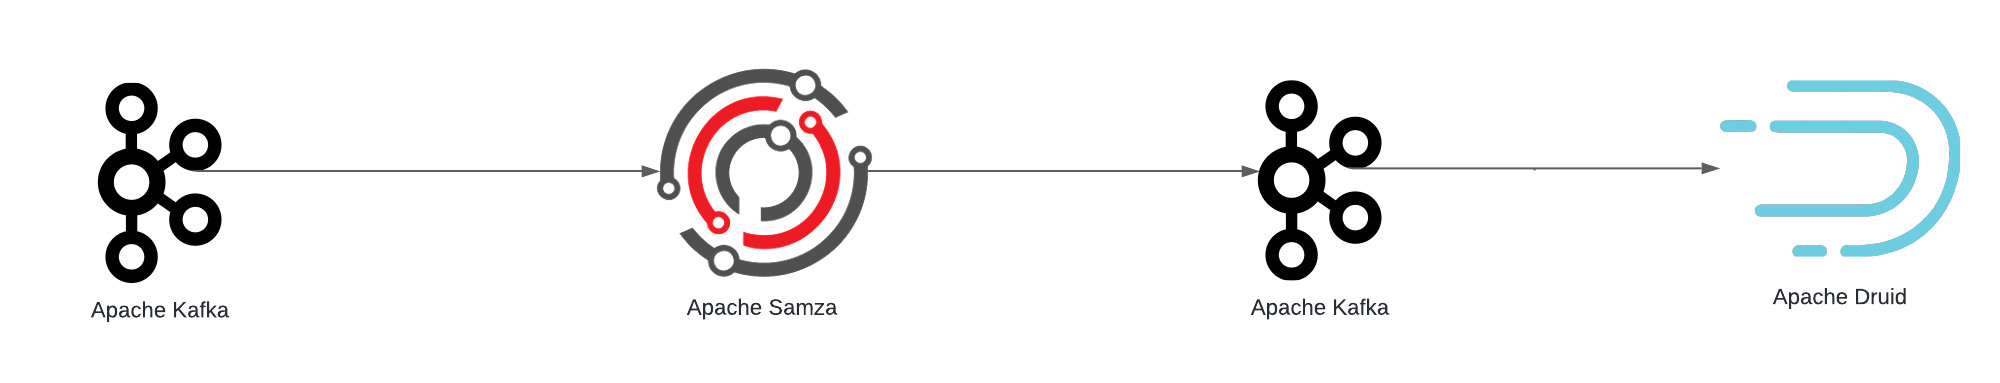
\includegraphics[width=0.8\textwidth]{teorico/KappaImplement.png}
\caption{Implementacion de la Arquitectura Kappa}
\label{fig:implementation_arquitectura_kappa}
\end{figure}

\subsection{Capacidades}
La Arquitectura Kappa ofrece varias capacidades clave:
\begin{itemize}
    \item \textbf{Simplificación}: Al unificar el procesamiento batch y en tiempo real, reduce la complejidad del sistema.
    \item \textbf{Consistencia}: Garantiza la coherencia entre los resultados del procesamiento en tiempo real y el reprocesamiento.
    \item \textbf{Escalabilidad}: Se adapta fácilmente al crecimiento del volumen de datos.
    \item \textbf{Reprocesamiento}: Permite actualizaciones sencillas de la lógica de procesamiento mediante el reprocesamiento del stream.
    \item \textbf{Latencia reducida}: Proporciona resultados en tiempo real con menos latencia que Lambda para la mayoría de los casos de uso.
\end{itemize}

\subsection{Debilidades}
A pesar de sus ventajas, la Arquitectura Kappa tiene algunas limitaciones:
\begin{itemize}
    \item \textbf{Complejidad tecnologica}: Requiere tecnologias con caracteristicas muy especificas en la capa de Stream Store.
    \item \textbf{Dependencia del almacenamiento}: Requiere un sistema de almacenamiento capaz de retener grandes volúmenes de datos históricos.
    \item \textbf{Complejidad}: Algunos análisis complejos pueden ser más difíciles de implementar en un modelo puramente basado en Streams.
\end{itemize}

\subsection{Conclusiones}
La Arquitectura Kappa representa una alternativa interesante en el diseño de sistemas de procesamiento de datos, 
ofreciendo una solución elegante para unificar el procesamiento batch y en tiempo real. 
Su enfoque en el procesamiento de streams como paradigma único simplifica la arquitectura general y reduce la complejidad del mantenimiento del código.

Mientras que es ideal para muchos casos de uso modernos de procesamiento de datos, 
especialmente aquellos que requieren resultados en tiempo real y flexibilidad en la actualización de la lógica de procesamiento, 
puede no ser la mejor opción para todos los escenarios.
\newpage